\documentclass[letterpaper,12pt]{article}
\usepackage[margin=.5in]{geometry}
\usepackage{graphicx}  % Include figure files
\usepackage{xcolor}  % Allow for a color text
\usepackage{amsmath}  % math fonts
\usepackage{amsfonts}  % math fonts
\usepackage{latexsym}  % math fonts
\usepackage{amssymb}  % math fonts
\usepackage{mathtools} % Give more control of how equations are displayed
\usepackage{appendix} % Lets you create an appendix
\usepackage[numbered]{matlab-prettifier} % Let's me import MATLAB code in a nice format
\usepackage{indentfirst} % This indents the first paragraph. By default latex won't do it.

%\setlength{\parskip}{1em} % This skips a line when making new paragraphs
\newtagform{show_eq}{(Eq.\ }{)}  % how the equation numbers are displayed
\usetagform{show_eq} % this goes with the \newtagform

\begin{document}

% ================================== Title Page ==========================================
\begin{titlepage}
 \begin{center}
 \vspace*{1in}
{\Huge Simulation of a Rotor with Gear Train Driving a Propeller}\\
    \bigskip
    by\\
    \bigskip
    {\Large Kevin Moran} \\
    \bigskip
    Date : November 1st, 2020

    \bigskip\bigskip\bigskip
    University of Southern California\\
    Aerospace and Mechanical Engineering Department\\
    AME 302 : System Dynamics
 \end{center}
\end{titlepage}

% ================================== Main Text =====================================

% --------------------------------- Impulse Images ---------------------------------
\begin{figure}[ht]
    \centering
    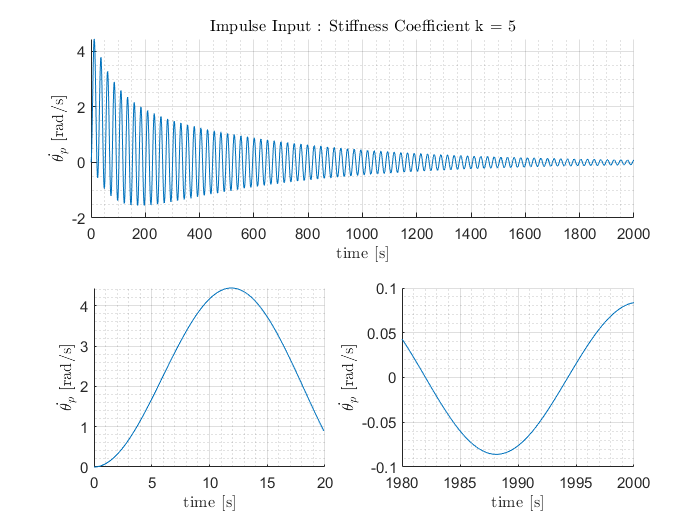
\includegraphics[scale = .8]{Images/Impulse_k5.png}
    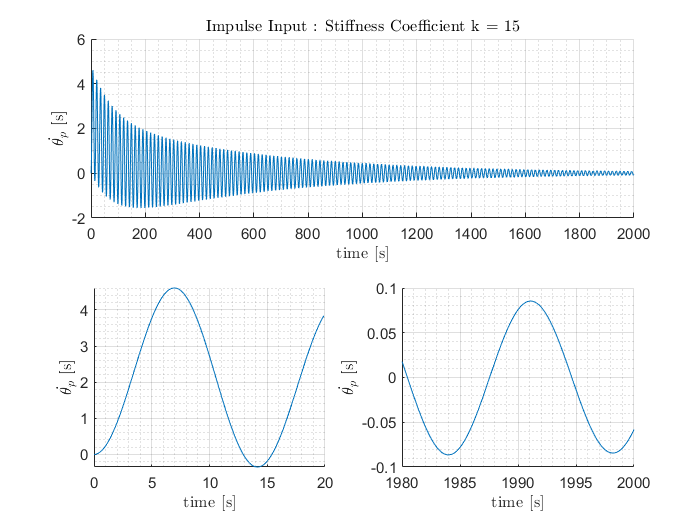
\includegraphics[scale = .8]{Images/Impulse_k15.png}
\end{figure}

\begin{figure}[ht]
    \centering
    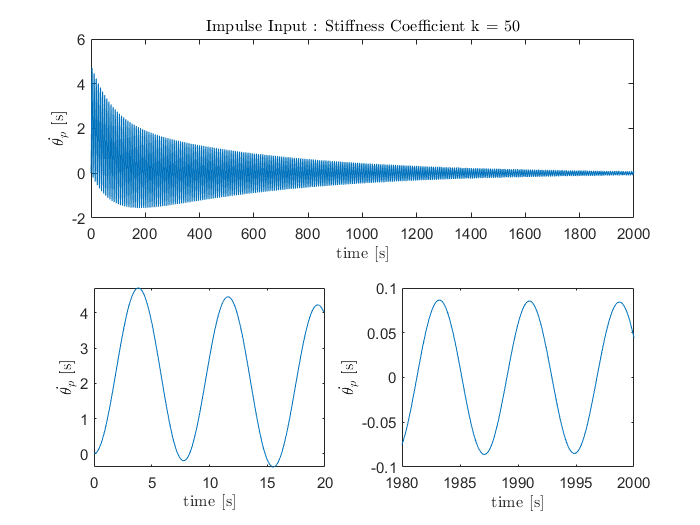
\includegraphics[scale = .8]{Images/Impulse_k50.png}
    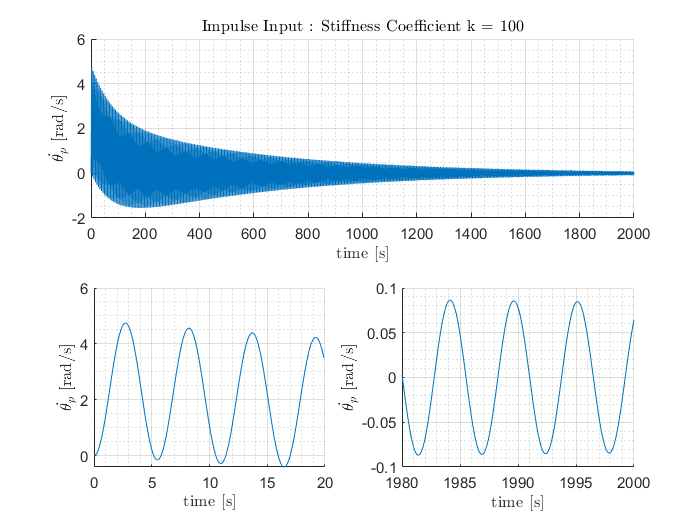
\includegraphics[scale = .8]{Images/Impulse_k100.png}
\end{figure}

\begin{figure}[ht]
    \centering
    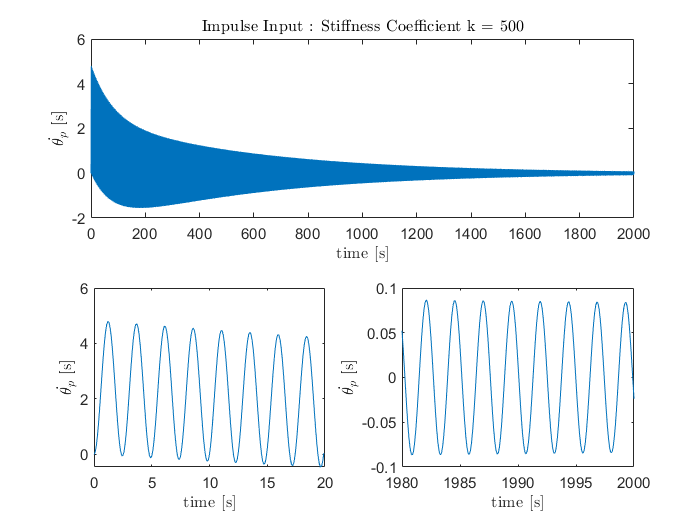
\includegraphics[scale = .8]{Images/Impulse_k500.png}
    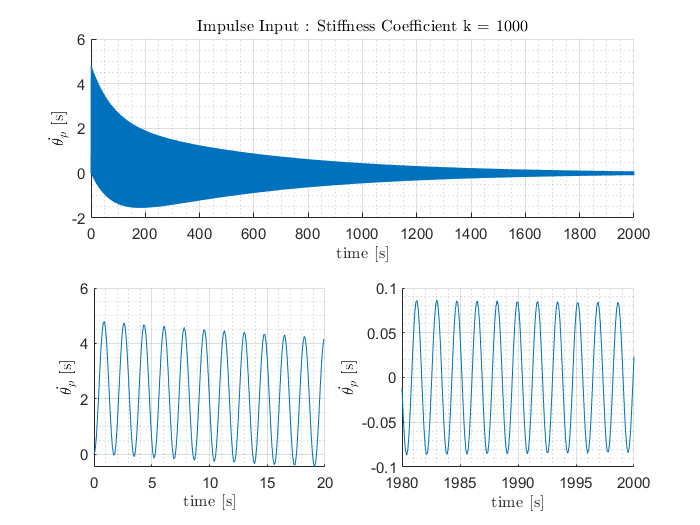
\includegraphics[scale = .8]{Images/Impulse_k1000.png}
\end{figure}

% --------------------------------- Step Images ---------------------------------
\begin{figure}[ht]
    \centering
    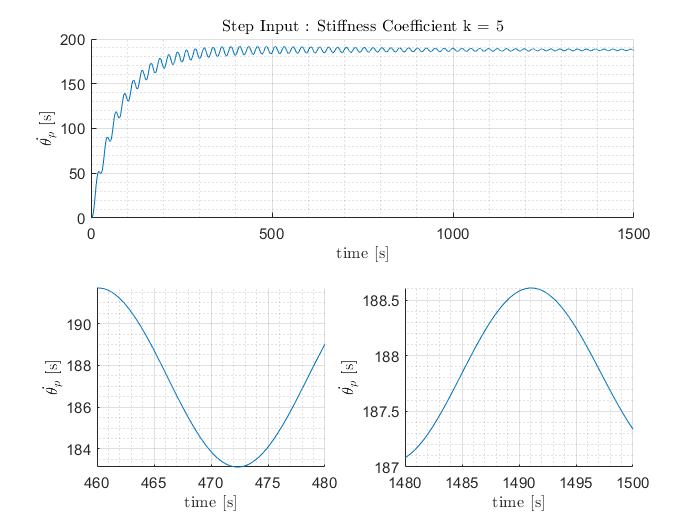
\includegraphics[scale = .8]{Images/StepInput_k5.png}
    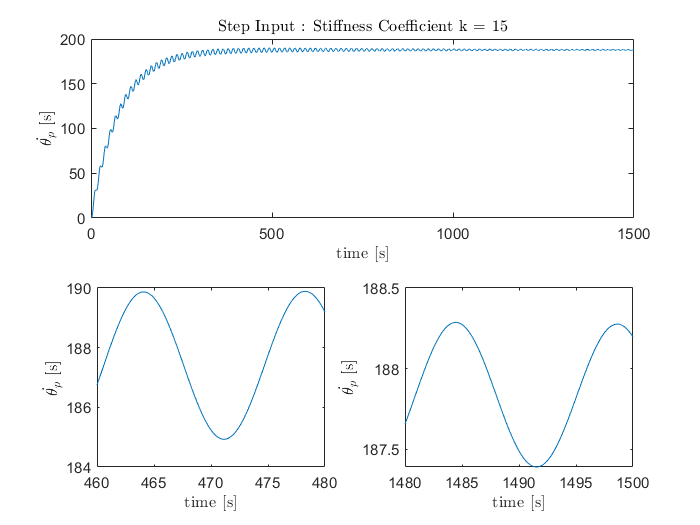
\includegraphics[scale = .8]{Images/StepInput_k15.png}
\end{figure}

\begin{figure}[ht]
    \centering
    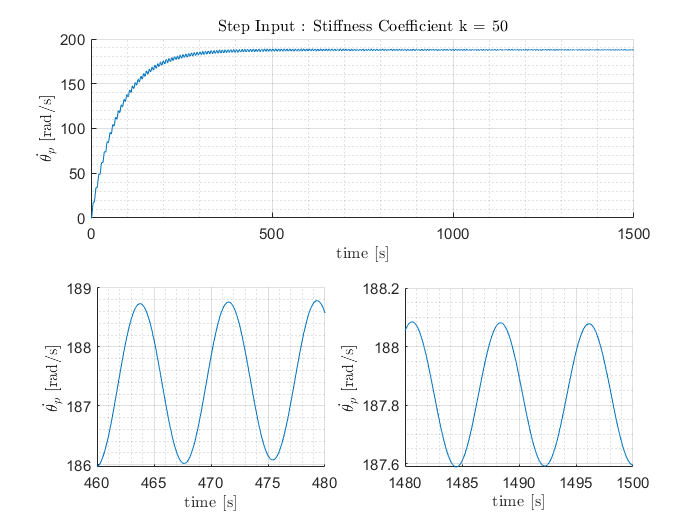
\includegraphics[scale = .8]{Images/StepInput_k50.png}
    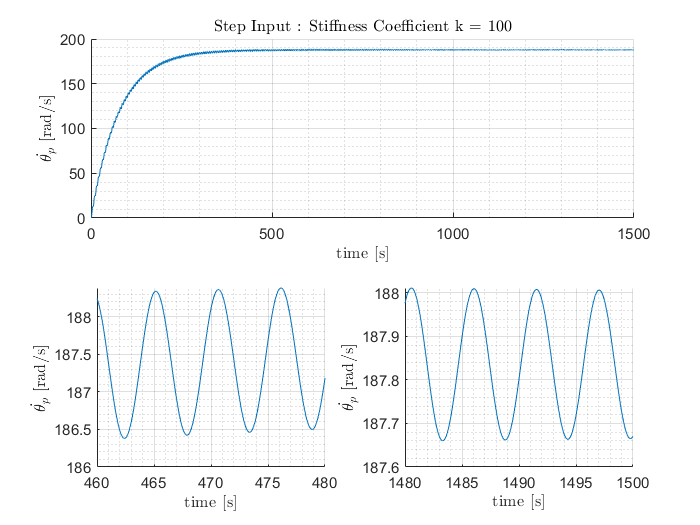
\includegraphics[scale = .8]{Images/StepInput_k100.png}
\end{figure}

\begin{figure}[ht]
    \centering
    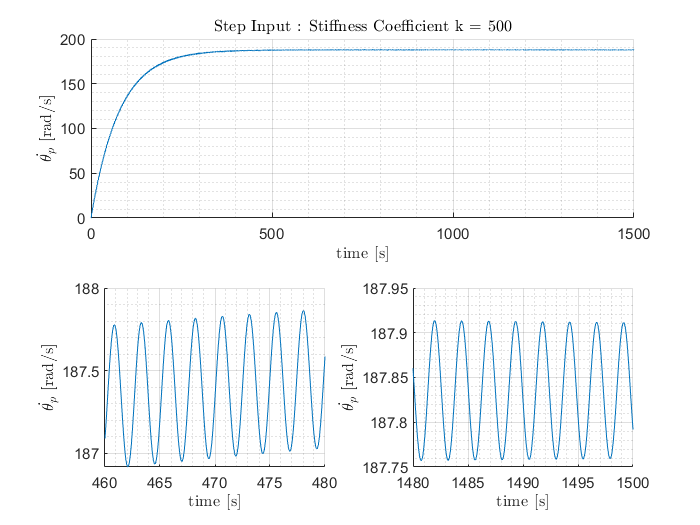
\includegraphics[scale = .8]{Images/StepInput_k500.png}
    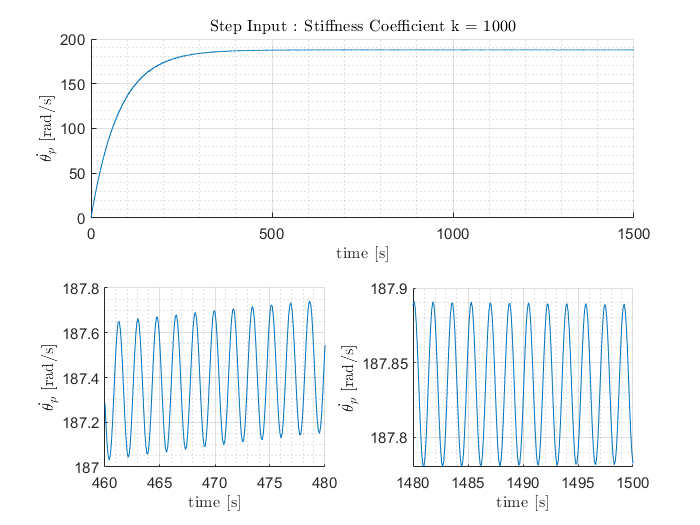
\includegraphics[scale = .8]{Images/StepInput_k1000.png}
\end{figure}

\end{document}